\chapter{Downsampling and Upsampling Images}
\label{chap:downsampling_and_upsampling}

\newcommand{\imghidden}{\ell_{\texttt{hidden}}}


\section{Introduction}

Changing the resolution of an image, or a feature map, is an operation you are likely to do many times, hence it will be worth expending some time understanding all its subtleties. Whether it is for resizing a picture, or to change the dimensionality of a representation, changing the sample-rate of a signal is a common operation. Resizing an image might seem like a trivial operation and often it is carelessly applied, producing results that are far from optimal. As discussed in the previous chapter, aliasing reduces the quality of the image. Aliasing is a visual phenomenon whereby the appearance of an image can change drastically after subsampling. In the previous chapter we discussed the case when the input is a continuous signal and the output is its discretized image.  


\section{Example: Aliasing-Based Adversarial Attack}

Aliasing in a system has consequences beyond the aesthetics of the final output. To illustrate the importance of aliasing when building vision systems in practice, let's consider the following simple system \cite{rodríguezmuñoz2022aliasing}:

\begin{align}
    u[n,m] &= \imgin \left[n,m\right] \circ \left[-1, 1 \right]  & \quad\quad \triangleleft \quad \texttt{conv}\\
    h[n,m] &= u[2n,2m]  & \quad\quad \triangleleft \quad \texttt{decimation}\\
    \imgout[n,m] &= \max (0,h[n,m])  & \quad\quad \triangleleft \quad \texttt{relu}
\end{align}

This system has three steps: the first step is a vertical edge filter (convolution of the input, $\imgin$, with a horizontal kernel, $[1, -1]$). The next step is to reduce the resolution of the filter output by taking one pixel every two along each dimension (this operation is called decimation). Decimation takes an input, $u$, with size $N\times M$, and outputs, $h$, with half the size $N/2 \times M/2$.
Finally, the third step is a relu nonlinearity.

\marginnote{A convolution followed by decimation is also called {\bf strided convolution} in the neural networks literature.}
\index{Strided convolution}

%\begin{equation}
%y \left[n,m\right]    =  \max (0, (x \left[n,m\right] \circ \left[-1, 1 \right] ) {\downarrow 2} )
%\end{equation}

As we will discuss in this chapter, the decimation step introduces {\bf aliasing}. As illustrated in \fig{\ref{figure:simple-network}}, an attacker could use aliasing in a system to infiltrate a signal hidden in the high-spatial frequencies that could change the output in unexpected ways. 
In this toy example, the construction of the attack is as follows. Let $\imgin \left[n,m\right]$ be the original image (e.g., a picture of a bird), and $\imghidden \left[n,m\right]$ be the hidden image (e.g., a picture of a stop sign). The attack $z \left[n,m\right]$ is given by
\begin{equation}
    \label{equation:aliasing-attack}
    z \left[n,m\right] = (-1)^n(-1)^m \imghidden \left[n,m\right]
\end{equation}
 
The attacked input image is $\imgin \left[n,m\right]+ \epsilon z \left[n,m\right]$, where $\epsilon$ is the chosen adversarial strength. In this example we used $\epsilon=0.05$. As we can see in \fig{\ref{figure:simple-network}}, the attacked input image is indistinguishable from the original input, $\imgin \left[n,m\right]$, and yet their outputs are completely different. The culprit for this bizarre effect is the strided convolution that samples the output for one pixel every two. An attacker with knowledge about it is able to construct a perturbation focused on manipulating the surviving samples (pixels at even rows and columns); the output at the discarded samples (pixels at an odd row or column) do not matter, or may even serve as extra degrees of freedom that can be used to make the attack less noticeable.




\begin{figure}[t]
	\centerline{
    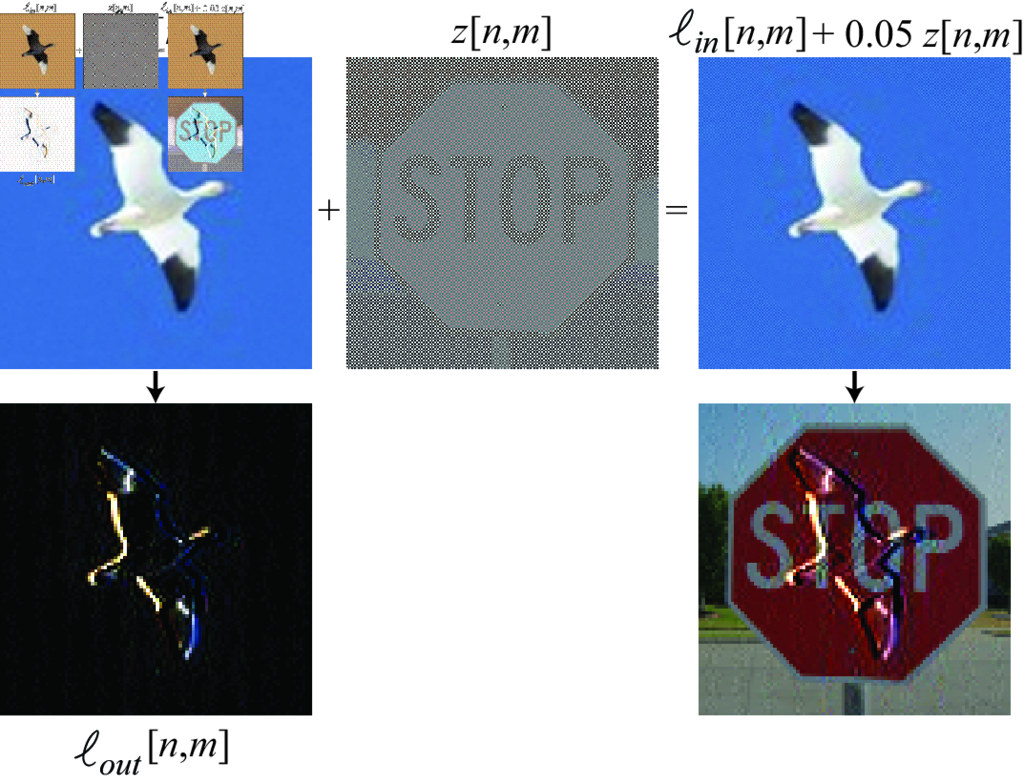
\includegraphics[width=0.8\linewidth]{figures/upsamplig_downsampling/toy_example_book2.eps}
    }
    \caption{Analytic aliasing-based attack of a toy system that computes the horizontal image gradient~\cite{rodríguezmuñoz2022aliasing}. Input image, $\imgin$, and  output image of $\imgout=\max(0, \imgin \circ_2 [1, -1])$, where $\circ_2$ denotes convolution with a stride of 2. As this simple system has aliasing, an attacker can inject a high frequency pattern, $z$, to change the output. Attacked image, $\imgin+z$, and the output after attack. It doesn't even look like a derivative!}
    \label{figure:simple-network}
\end{figure}


In this chapter we will study aliasing when manipulating image resolution and how to reduce it. 


\section{Downsampling}

Downsampling is an operation that consists of reducing the resolution of an image. When we reduce the resolution, some information will be lost; specifically fine image details will be lost. But carelessly removing pixels will produce a greater loss of information than necessary. The goal of this chapter will be to study how downsampling has to be done to minimize the amount of information lost.  


\subsection{Decimation}

Image decimation consists of changing the resolution of an image by dropping samples. Decimation of an image of size $N \times M$ by a factor of $k$, where $N$ and $M$ are divisible by $k$, results in a lower resolution image of size $N/k \times M/k$: 
\begin{equation}
%y \left[n,m\right]    =  
\img_{\downarrow k} \left[n,m\right]  = \img \left[kn, km\right]
\end{equation}
It is common to use the notations $\img_{\downarrow k} \left[n,m\right]   = \img \left[n,m\right] \downarrow k = \img \left[kn,km\right]$ to denote the decimation operator by a factor $k$. Decimation could be different across each dimension, but for the analysis here we will assume that both dimensions are treated equally, as it is usually done. 

\marginnote{Decimation is often drawn using the following block:
~\\
%\begin{figure}[h!]
\begin{center}
\tikzstyle{int}=[draw, minimum size=3em]
\tikzstyle{init} = [pin edge={to-,thin,black}]
\begin{tikzpicture}[node distance=0cm,auto,>=latex']
  \node [int] (box1) {$\downarrow k$};
   \node [left of=box1,node distance=1.1cm] (input) {$\img$};
   \node [right of=box1,node distance=1.3cm] (output) {$\img_{\downarrow k}$};
    \node (c) [right of=box1,node distance=3cm, coordinate] {};
    \path[->] (input) edge node {} (box1);
    \path[->] (box1) edge node {} (output);
\end{tikzpicture}
\end{center}
%\label{fig:genericfilterH}
%\end{figure}
}

Decimation is a linear operation therefore we can write it as a matrix. In the one-dimensional (1D) case, for a signal of length 8, subsampling by a factor of 2 can be described by the following linear operator:
\begin{equation}
\mathbf{D}_2 = \left[ 
\begin{array}{cccccccc}
1 & 0 & 0 & 0 & 0 & 0 & 0 & 0\\
0 & 0 & 1 & 0 & 0 & 0 & 0 & 0\\
0 & 0 & 0 & 0 & 1 & 0 & 0 & 0\\ 
0 & 0 & 0 & 0 & 0 & 0 & 1 & 0 
\end{array}
\right]
\end{equation}


The \fig{\ref{fig:subsampled_textures}} shows an example of a picture and two decimated images with factors $k=2$ and $k=4$. For visualization purposes, the images are scaled so that they occupy the same area.
%\vspace{-0.2in}
\begin{figure}[h]
\centerline{
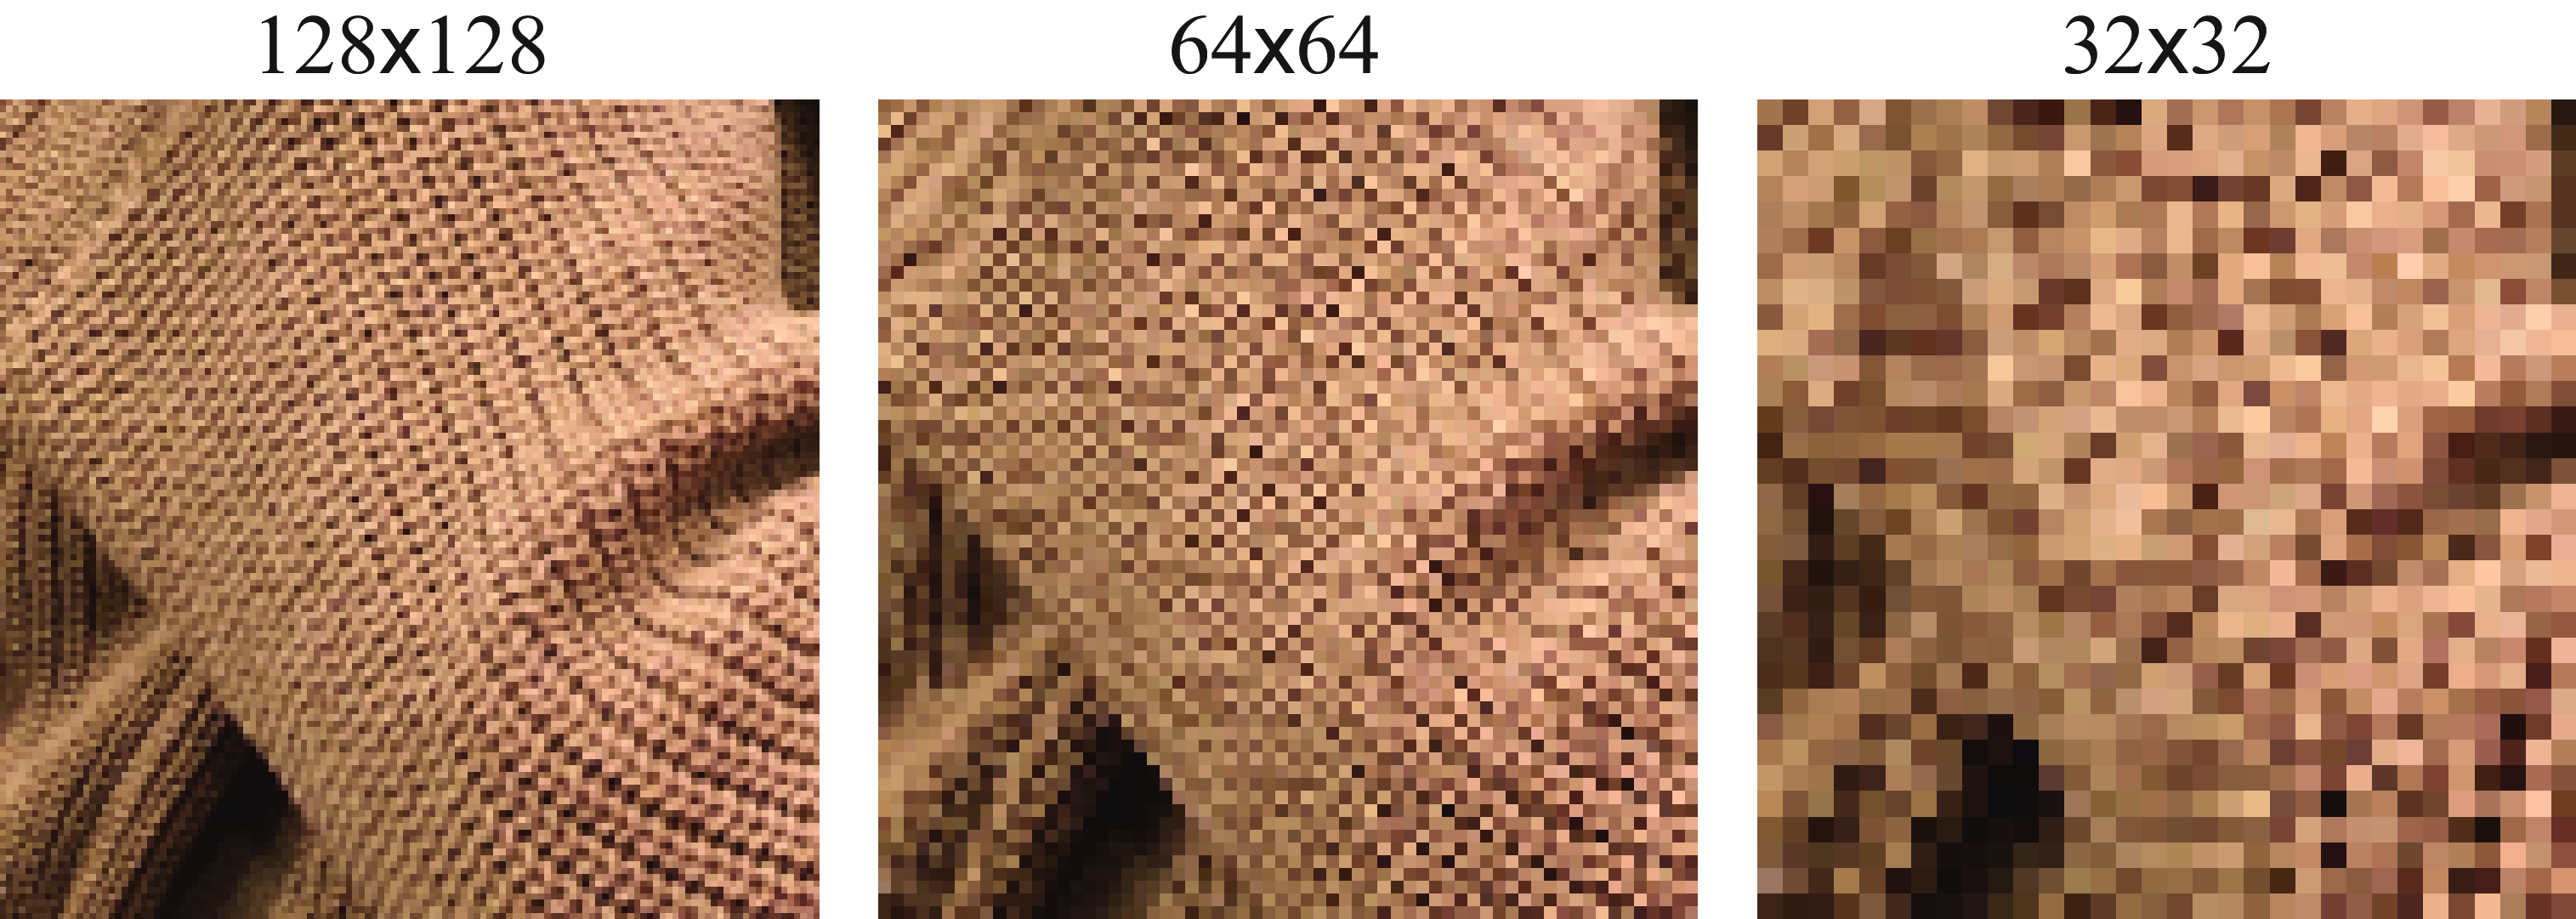
\includegraphics[width=1\linewidth]{figures/upsamplig_downsampling/subsampled_textures.eps}
}
\caption{Input image (left) and two decimated versions of the same image with factors $k=2$ and $k=4$.}
\label{fig:subsampled_textures}
\end{figure}
%\vspace{-0.2in}

As we downsample the image, we lose details in the texture such as the orientation of the knitting, and it becomes harder to see the overall shape. Just reducing resolution by a factor of 4 results in an almost unintelligible image. The loss of information is due to the reduced resolution, but most important, in this example, additional information is lost due to aliasing. Aliasing has introduced new texture features in the subsampled image that are not present in the original image and that could have been avoided.

How can we reduce the resolution of an image while preserving as many details as possible?


\subsection{Decimation in the Fourier Domain}


As we did before for the continuous case, analyzing how the decimation operator affects the signal in the Fourier domain can be very revealing. 
In this section we compute the relationship between the Fourier transform (FT) of the original image, $\img$ and the sampled one, $\img_{\downarrow k}$. We will use the finite length discrete Fourier transform (DFT). If the DFT of $\img \left[n,m\right]$ is $\capitalimg \left[u,v\right]$, the DFT of the sampled image, $\img \left[kn,km\right]$ (with size $N/k \times M/k$), is:
\begin{equation}
\capitalimg_{\downarrow k} \left[u,v\right]   = \sum_{n=0}^{N/k-1} \sum_{m=0}^{M/k-1} \img \left[kn,km\right] \exp{ \left(  -j2\pi \frac{nu}{N/k} \right)}  \exp{ \left(  -j2\pi \frac{mv}{M/k} \right)}
\label{eq:down1}
\end{equation}
as before, we can define an image, $\img_{\delta_k} \left[n,m\right]$, of same size as the input image, $N \times M$, where we set to zero the samples that will be removed in the decimation operation:
\begin{eqnarray}
\img_{\delta_k} \left[n,m\right] &=& \img \left[n,m\right] \sum_{s=0}^{N/k-1} \sum_{r=0}^{M/k-1} \delta \left[n - sk \, ,m - rk \right] \\
&=&  \img \left[n,m\right]  \delta_k \left[n,m\right] 
\label{eq:down2}
\end{eqnarray}
where $\delta_k \left[n,m\right]$ is the discrete version of the {\bf delta train}. Using $\img_{\delta_k}$ we can rewrite \eqn{\ref{eq:down1}}, with a change of the summation indices, as:
\begin{equation}
\capitalimg_{\downarrow k} \left[u,v\right]   = \sum_{n=0}^{N-1} \sum_{m=0}^{M-1} \img_{\delta_k} \left[n,m\right] \exp{ \left(  -j2\pi \frac{nu}{N} \right)}  \exp{ \left(  -j2\pi \frac{mv}{M} \right)}
\end{equation}

Therefore, the DFT of $\img\left[kn,km\right]$ is the DFT of $\img_{\delta_k} \left[n,m\right]$, which is the product of two signals, \eqn{\ref{eq:down2}}. The first term is $\img \left[n,m\right]$, and the second term is a discrete delta train (also called the Kronecker comb): 
\begin{equation}
\delta_k \left[n,m\right]  =  \sum_{s=0}^{N/k-1} \sum_{r=0}^{M/k-1} \delta \left[n - sk \, ,m - rk \right]
\end{equation}
The DFT of the discrete delta train, when $M$ and $N$ are divisible by $k$, is:
\begin{equation}
\Delta_k \left[u,v\right]  = \frac{NM}{k^2}  \sum_{s=0}^{k-1} \sum_{r=0}^{k-1} \delta \left[u - s\frac{N}{k} \, ,v - r\frac{M}{k} \right]
\end{equation}

This definition is valid for frequencies inside the interval $[u,v] \in [0,N-1]\times[0,N-1]$. Outside of that interval, we will have its periodic extension. 

\Fig{\ref{fig:discrete_delta_train}} shows $\delta_k \left[n,m\right]$ and its Fourier transform, $\Delta_k \left[u,v\right]$, in the bottom, for images size of $32 \times 32$ pixels. For the FT we  plot signals using an interval that puts the frequency $[0,0]$ in the center. 

\begin{figure}[t]
\centerline{
\includegraphics[width=1\linewidth]{figures/upsamplig_downsampling/discrete_delta_train.eps}
}
\caption{(top) Visualization of three discrete two-dimensional (2D) delta trains with $k=2,4,8$. (bottom) Corresponding DFTs. The DFT of a delta train is another delta train.}
\label{fig:discrete_delta_train}
\end{figure}


Now we are ready to write the DFT of $x_{\delta_k} \left[n,m\right]$. This is the DFT of the product of two images, \eqn{\ref{eq:down2}}, so we can apply the dual of the circular convolution theorem for finite length discrete signals (where both signals are extended periodically):
\begin{eqnarray}
\label{eq:decimationFT}
\capitalimg_{\downarrow k} \left[u,v\right] &=& \frac{1}{NM} \capitalimg \left[u,v\right] \circ \Delta_k \left[u,v\right] \\ \nonumber
&=& \frac{1}{k^2} \sum_{s=0}^{k-1} \sum_{r=0}^{k-1} \capitalimg \left[u - s\frac{N}{k} \, ,v - r\frac{M}{k} \right]
\end{eqnarray}
The DFT of the sampled image by a factor $k$ is the superposition of $k \times k$ shifted copies of the DFT of the original image. Each copy is centered on one of the deltas in $\Delta_k \left[u,v\right]$.

The images in \fig{\ref{fig:discrete_texture_sampling}} show $\img_{\delta_k} \left[n,m\right]$ and $\capitalimg_{\downarrow k} \left[u,v\right]$. The original image, $\img \left[n,m\right]$, is $128 \times 128$. The DFT of the sampled image, $\img_{\downarrow k} \left[n,m\right]$, is the inner window with size $N/2k \times M/2k$ (shown as a green square).

\begin{figure}[h]
\centerline{
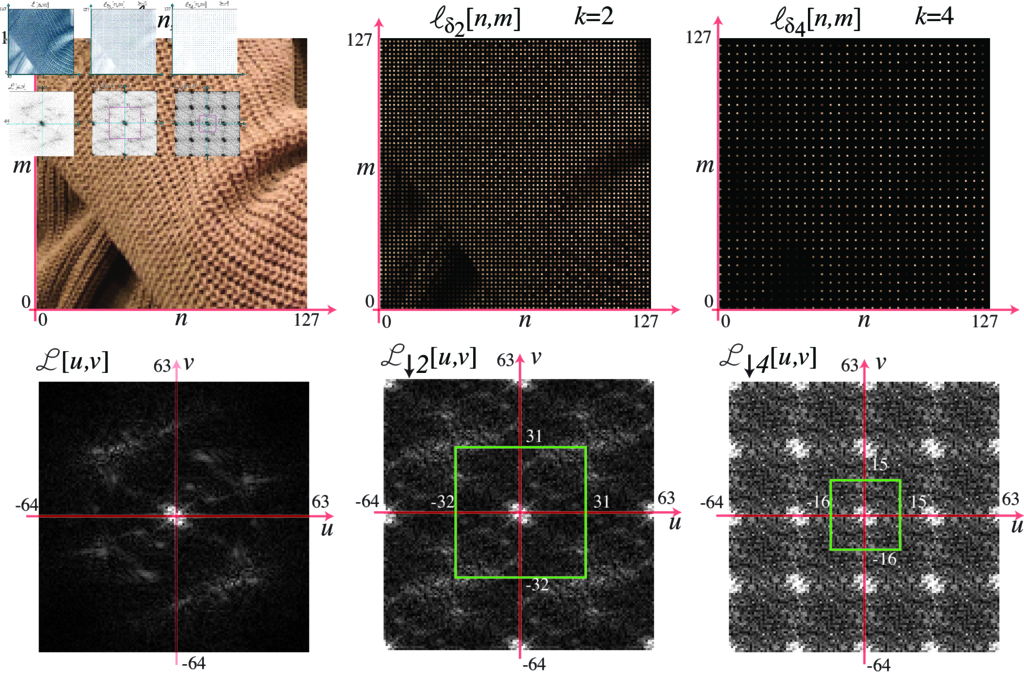
\includegraphics[width=1\linewidth]{figures/upsamplig_downsampling/discrete_texture_sampling2.eps}
}
\caption{(top) Visualization of an image multiplied by delta trains, and (bottom) and their corresponding DFTs. Only the DFT magnitude is shown.}
\label{fig:discrete_texture_sampling}
\end{figure}

In the case of $k=2$, it is useful to see how the spectrum of the decimated signal is obtained. As shown from \eqn{\ref{eq:decimationFT}}, the resulting spectrum is a sum of shifted versions of the original spectrum, $\capitalimg \left[u,v\right]$, as shown in \fig{\ref{fig:components_aliasing_FT}}. The image shows the four copies that are summed to obtain the decimated spectrum:


%\vspace{-.2in}
\begin{figure}[h]
\centerline{
\includegraphics[width=1\linewidth]{figures/upsamplig_downsampling/components_aliasing_FT2.eps}
}
\caption{DFT of an image multiplied by a delta train and the decomposition into the four different translated copies of the DFT of the original input image.}
\label{fig:components_aliasing_FT}
\end{figure}
%\vspace{-.2in}

The first component is $\capitalimg \left[u,v\right]$, the three other copies are shifted versions of $\capitalimg \left[u,v\right]$. Shifting is equivalent to a circular shift as $\capitalimg \left[u,v\right]$ is periodic in $u$ and $v$. All the spectral content inside the green box in the shifted copies will produce aliasing after decimation. 

\subsection{Aliasing in Matrix Form}

%Using the matrix forms of the decimation, DFT and the inverse DFT operators, we can get a more visual explanation of aliasing. In 1D, these operators are easy to visualize. 

We can provide another description of decimation and aliasing using the matrix form of the decimation and DFT operators. As decimation and the Fourier transform are linear operators, we can write them as matrices. 
This description will provide a different visualization for the same phenomena described in the previous section. For simplicity of the visualizations we will work with 1D signals, but the same can be extended to 2D.

Using matrices, we can write decimation as $\boldimg_{\downarrow 2} = \mathbf{D}_2 \boldimg$. We use the Fourier matrices $\mathbf {F}_{N}$ and $1/N \mathbf {F}^{*}_{N}$ to denote the DFT and its inverse  (which is the complex conjugate of the DFT) for signals of length $N$. Using this notation, the relationship between the original spectrum $\capitalimg \left[u\right]$ and the sampled version, $\capitalimg_{\downarrow 2} \left[u\right]$, is:
\begin{equation}
\boldcapitalimg_{\downarrow 2} = \frac{1}{N} \mathbf{F}_{N/2} \mathbf{D}_2 \mathbf{F}^{*}_{N} \boldcapitalimg
\label{eq:matrixformsubsampling}
\end{equation}

One interesting property of the Fourier matrix is that $\mathbf{D}_2 \mathbf{F}_{N} = [\mathbf{F}_{N/2} ~|~ \mathbf{F}_{N/2}]$. The matrix $\mathbf{D}_2$ selects all the odd rows of the matrix $\mathbf{F}_{N}$ and ignores the even ones. Therefore, 
\begin{eqnarray}
\frac{1}{N} \mathbf{F}_{N/2} \mathbf{D}_2 \mathbf{F}^{*}_{N} &=& \frac{1}{N}\mathbf{F}_{N/2}  [\mathbf{F^*}_{N/2} ~|~ \mathbf{F^*}_{N/2}] \\
&=& \frac{1}{N} \frac{N}{2} [\mathbf{I}_{N/2} ~|~ \mathbf{I}_{N/2}] \\
&=& \frac{1}{2} [\mathbf{I}_{N/2} ~|~ \mathbf{I}_{N/2}]
\end{eqnarray}
where $\mathbf{I}_{N/2}$ is the identity matrix of size $N/2 \times N/2$. Replacing this result inside \eqn{\ref{eq:matrixformsubsampling}} gives the following relationship between the DFT of the original signal and the subsampled one:
\begin{equation}
\boldcapitalimg_{\downarrow 2} = \frac{1}{2} [\mathbf{I}_{N/2} ~|~ \mathbf{I}_{N/2}] \boldcapitalimg
\end{equation}
This equation is analogous to \eqn{\ref{eq:decimationFT}} with $k=2$ and for 1D signals.

In 1D, we can visualize these operators which helps to make the previous derivations intuitive. For 1D signals of length $N=16$, \eqn{\ref{eq:matrixformsubsampling}} has the visual form shown in \fig{\ref{fig:aliasing_in_matrix_form}}:
%\vspace{-.2in}
\begin{figure}[h!]
\centerline{
\includegraphics[width=.9\linewidth]{figures/upsamplig_downsampling/aliasing_in_matrix_form.eps}
}
\caption{Visual representation of \eqn{\ref{eq:matrixformsubsampling}}.}
\label{fig:aliasing_in_matrix_form}
\end{figure}
%\vspace{-.2in}

Note that for the matrices $\mathbf{F}_{N}$ used here, we are not using the convention of putting the frequency 0 in the middle as this makes visualizations in matrix form easier. 

The product between the decimation matrix and the inverse DFT, $\mathbf{D}_2 \mathbf{F^*}_{16}$, is (\fig{\ref{fig:decimationFT_inmatrixform}}):
%\vspace{-.2in}
\begin{figure}[h!]
\centerline{
\includegraphics[width=.9\linewidth]{figures/upsamplig_downsampling/decimationFT_inmatrixform.eps}
}
\caption{Visualization of the product $\mathbf{D}_2 \mathbf{F^*}_{16}$ and its result.}
\label{fig:decimationFT_inmatrixform}
\end{figure}
%\vspace{-.2in}

In \fig{\ref{fig:decimationFT_inmatrixform}} we can see how the odd rows of $\mathbf{F^*}_{16}$ gives a new sub matrix composed of two identical blocks. Interestingly, each of those two blocks are identical to $\mathbf{F^*}_{8}$. A similar structure emerges also when applying $\mathbf{D}_4$. Combining these last equations together, we get the final result:
%\vspace{-.2in}
\begin{figure}[h!]
\centerline{
\includegraphics[width=0.9\linewidth]{figures/upsamplig_downsampling/decimation_finalequations_inmatrixform2.eps}
}
\caption{Visualization of decimation and aliasing.}
\label{fig:decimation_finalequations_inmatrixform}
\end{figure}
%\vspace{-.2in}

This last result shows visually how aliasing happens. Each component of the final DFT, $\capitalimg_{\downarrow 2} \left[u\right]$, is the sum of two of the components of $\capitalimg \left[u\right]$. For instance, $\capitalimg_{\downarrow 2} \left[0\right] = 0.5 \capitalimg \left[0\right] + 0.5 \capitalimg \left[8\right]$. Both components are mixed in the final result. 

In the next subsection we will discuss anti-aliasing filters. Anti-aliasing consists in setting to zero, before decimation, the $N/k$ the spectral components that produce aliasing. 

\subsection{Anti-Aliasing Filters}

Anti-aliansing filtering is an essential operation whenever we manipulate the resolution of an image. When decimating a signal of size $N \times N$ with a scaling factor $k$, aliasing is produced by all the content at frequencies that are above $u,v > N/2k$. Therefore, to reduce aliasing, we have to remove any spectral content of the signal present at high spatial frequencies. We will do so by using an anti-aliasing filter that will blur the image before downsampling. Blurring removes high-spatial frequencies in the image. 

The ideal anti-aliasing filter is a box in the Fourier domain with a cut-off frequency of $L=N/(2k)$ (using the notation introduced in \chap{\ref{chapter:sampling}}). The inverse Fourier transform of a box in the frequency domain, with width $2L+1=N/k+1$, is the {\bf discrete sinc} function of length $N$ in the spatial domain:
\begin{equation}
\frac{1}{N} \frac 
{\sin(\pi n (N/k+1)/N)}
{\sin(\pi n/N)}
\xrightarrow{\mathscr{F}} 
box_{N/2k} \left[ u \right]
\end{equation}
\index{Discrete sinc}

In 2D, the ideal anti-aliasing filter is separable and is obtained by two consecutive 1D convolutions along each dimension. The discrete sinc is very similar to the continuous sinc described in \chap{\ref{chapter:sampling}}. The discrete sinc is periodic, with period $N$. The following plot (\fig{\ref{fig:discretesinc}}) shows the anti-aliasing sinc for $N=32$ and $k=2$ and the magnitude of its Fourier transform:
\newpage 

%\vspace{-.2in}
\begin{figure}[h!]
\centerline{
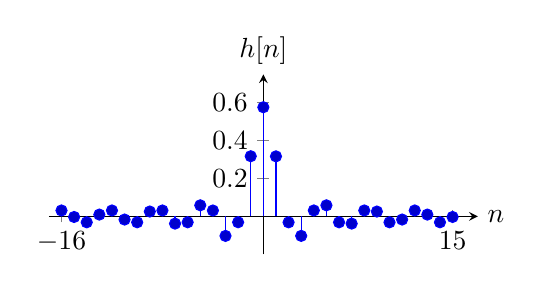
\begin{tikzpicture}
\begin{axis} [width=200pt,height=110pt,
	axis x line=middle, 
	axis y line=middle, 
	tick align=center,
	every axis x label/.style={at={(current axis.right of origin)},anchor=west},
	every axis y label/.style={at={(current axis.above origin)}, anchor=north east,above=0mm},
	xmin=-17, xmax=17,
	xtick={-16,15},
	xlabel=$n$,
	ymin=-0.2, ymax=0.75,
	ytick={0, 0.2,0.4, 0.6},
	ylabel={$h [n]$},
	color=black]
 \addplot+[ycomb][domain=-16:15,samples=32,samples y=0] 
 ({x}, {1/32*sin(deg(pi*(x+0.001)*(32/2+1)/32)) / sin(deg(pi*(x+0.001)/32))  });
\end{axis}
\end{tikzpicture}
%\centerline{
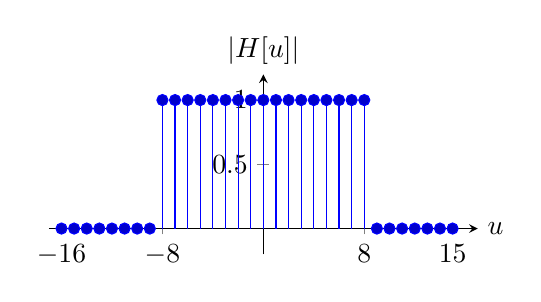
\begin{tikzpicture}
\begin{axis} [width=200pt,height=110pt,
	axis x line=middle, 
	axis y line=middle, 
	tick align=center,
	every axis x label/.style={at={(current axis.right of origin)},anchor=west},
	every axis y label/.style={at={(current axis.above origin)}, anchor=north east,above=0mm},
	xmin=-17, xmax=17,
	xtick={-16,-8,0,8,15},
	xlabel=$u$,
	ymin=-0.2, ymax=1.2,
	%ytick={-7,...,7},
	ylabel={$\left| H [u] \right|$},
	color=black]
 \addplot+[ycomb][domain=-16:15,samples=32,samples y=0] 
 ({x}, {abs(x)<32/(2*2)+1});
\end{axis}
\end{tikzpicture}
}
\caption{Discrete sinc function for $N=32$ and $k=2$ and the magnitude of its DFT.}
\label{fig:discretesinc}
\end{figure}
\vspace{-.1in}

And for $k=4$, the impulse response becomes wider and its Fourier transform has a lower cut-off frequency, $N/2k = 4$:

\vspace{-.2in}
\begin{figure}[h!]
\centerline{
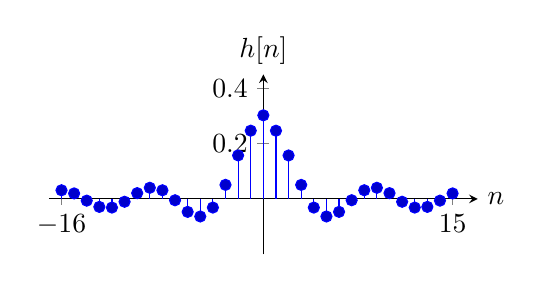
\begin{tikzpicture}
\begin{axis} [width=200pt,height=110pt,
	axis x line=middle, 
	axis y line=middle, 
	tick align=center,
	every axis x label/.style={at={(current axis.right of origin)},anchor=west},
	every axis y label/.style={at={(current axis.above origin)}, anchor=north east,above=0mm},
	xmin=-17, xmax=17,
	xtick={-16,15},
	xlabel=$n$,
	ymin=-0.2, ymax=0.45,
	ytick={0, 0.2,0.4},
	ylabel={$h [n]$},
	color=black]
 \addplot+[ycomb][domain=-16:15,samples=32,samples y=0] 
 ({x}, {1/32*sin(deg(pi*(x+0.001)*(32/4+1)/32)) / sin(deg(pi*(x+0.001)/32))  });
\end{axis}
\end{tikzpicture}
%\centerline{
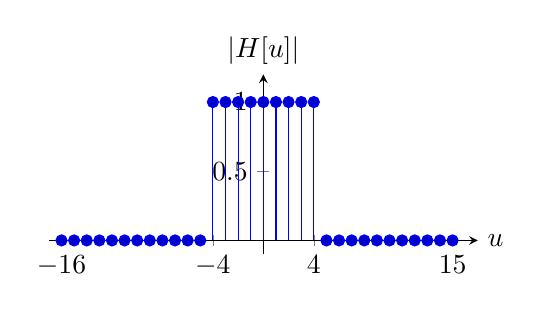
\begin{tikzpicture}
\begin{axis} [width=200pt,height=110pt,
	axis x line=middle, 
	axis y line=middle, 
	tick align=center,
	every axis x label/.style={at={(current axis.right of origin)},anchor=west},
	every axis y label/.style={at={(current axis.above origin)}, anchor=north east,above=0mm},
	xmin=-17, xmax=17,
	xtick={-16,-4,0,4,15},
	xlabel=$u$,
	ymin=-0.1, ymax=1.2,
	%ytick={-7,...,7},
	ylabel={$\left| H [u] \right|$},
	color=black]
 \addplot+[ycomb][domain=-16:15,samples=32,samples y=0] 
 ({x}, {abs(x)<32/(2*4)+1});
\end{axis}
\end{tikzpicture}
}
\caption{Discrete sinc function for $N=32$ and $k=4$ and the magnitude of its DFT.}
\label{fig:discretesinc_k4}
\end{figure}
\vspace{-.2in}



One disadvantage of the ideal anti-aliasing filter is that the it requires convolving the image with a very large filter (as large as the image). We would like to use smaller filters to reduce the computational cost. 
One method to design anti-aliasing filters with a finite impulse response is to use a window, $w [n]$, and to use as anti-aliasing filter the kernel $w [n] h[n]$, where $h[n]$ is the impulse response of the ideal anti-aliasing filter. Typical windows used are the rectangular, Hamming, Parzen, or Kaiser windows. 

The rectangular window sets to zero all the values outside of the interval $\left[-L, L\right]$. When $L=5$, it gives a tap-11 filter (a filter with an impulse response of length 11) with the following profile:

%\begin{equation}
%h= [0.054, 0.029, -0.096, -0.029, 0.295, 0.493, 0.295, -0.029, -0.096, 0.029, 0.054]
%\end{equation}

\vspace{-.1in}
\begin{figure}[h!]
\centerline{
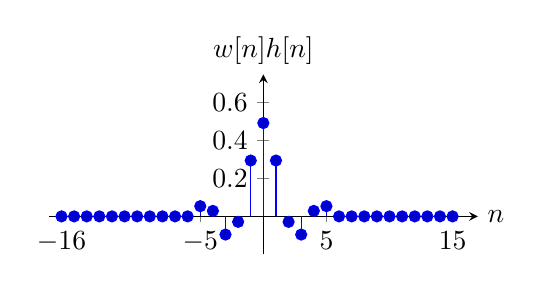
\begin{tikzpicture}
\begin{axis} [width=200pt,height=110pt,
	axis x line=middle, 
	axis y line=middle, 
	tick align=center,
	every axis x label/.style={at={(current axis.right of origin)},anchor=west},
	every axis y label/.style={at={(current axis.above origin)}, anchor=north east,above=0mm},
	xmin=-17, xmax=17,
	xtick={-16,-5, 5, 15},
	xlabel=$n$,
	ymin=-0.2, ymax=0.75,
	ytick={0, 0.2,0.4, 0.6},
	ylabel={$w [n] h[n]$},
	color=black]
\addplot+[ycomb] plot coordinates {(-16, 0.000) (-15, -0.000) (-14, -0.000) (-13, 0.000) (-12, 0.000) (-11, -0.000) (-10, -0.000) (-9, 0.000) (-8, 0.000) (-7, -0.000) (-6, -0.000) (-5, 0.054) (-4, 0.029) (-3, -0.096) (-2, -0.029) (-1, 0.295) (0, 0.493) (1, 0.295) (2, -0.029) (3, -0.096) (4, 0.029) (5, 0.054) (6, -0.000) (7, -0.000) (8, 0.000) (9, 0.000) (10, -0.000) (11, -0.000) (12, 0.000) (13, 0.000) (14, -0.000) (15, -0.000)};
\end{axis} 
\end{tikzpicture}
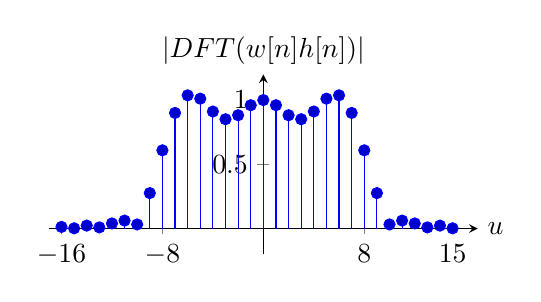
\begin{tikzpicture}
\begin{axis} [width=200pt,height=110pt,
	axis x line=middle, 
	axis y line=middle, 
	tick align=center,
	every axis x label/.style={at={(current axis.right of origin)},anchor=west},
	every axis y label/.style={at={(current axis.above origin)}, anchor=north east,above=0mm},
	xmin=-17, xmax=17,
	xtick={-16,-8,0,8,15},
	xlabel=$u$,
	ymin=-0.2, ymax=1.2,
	ylabel={$\left| DFT(w [n] h[n]) \right|$},
	color=black]
 \addplot+[ycomb]  plot coordinates {(-16, 0.013) (-15, 0.002) (-14, 0.023) (-13, 0.009) (-12, 0.040) (-11, 0.062) (-10, 0.032) (-9, 0.276) (-8, 0.609) (-7, 0.900) (-6, 1.037) (-5, 1.011) (-4, 0.911) (-3, 0.851) (-2, 0.882) (-1, 0.960) (0, 1.000) (1, 0.960) (2, 0.882) (3, 0.851) (4, 0.911) (5, 1.011) (6, 1.037) (7, 0.900) (8, 0.609) (9, 0.276) (10, 0.032) (11, 0.062) (12, 0.040) (13, 0.009) (14, 0.023) (15, 0.002)};
\end{axis}
\end{tikzpicture}
}
\caption{Kernel $w [n] h[n]$, where $h[n]$ is a sinc and $w [n]$ is a rectangular window of length 11.}
%\label{fig:discretesinc}
\end{figure}
%\vspace{-.2in}

The Fourier transform of the windowed impulse response, $w [n] h[n]$, is the convolution of Fourier transforms. The Fourier transform of the rectangular window is a sinc function. Therefore, the resulting Fourier transform is the convolution of the rectangle with the sinc function, which produces a smooth rectangle with some oscillations. Using other windows allows trading off the smoothing of the ideal rectangular form of the ideal low-pass filter and the oscillations. 

The {\bf Hamming window} is defined as:
\index{Hamming window}
\begin{equation}
w  \left[n\right] =  \begin{cases}
    0.54+0.46 \cos (\pi n/L)     & \quad \text{if }  n \in  \left[-L, L\right] \\
    0       & \quad \text{otherwise }\\
\end{cases}
\end{equation}
The Hamming window ($L=5$) produces a smooth transfer function with oscillations of smaller amplitude in the Fourier domain:
\begin{equation}
h = [1, 0.65, -2.45, -0.82, 8.8, 15, 8.8, -0.82, -2.45, 0.65, 1] / 29.36
\end{equation}

% /Users/antoniotorralba/atb/BOOK/code/aliasing/filters_for_antialising.m
\vspace{-.2in}
\begin{figure}[h!]
\centerline{
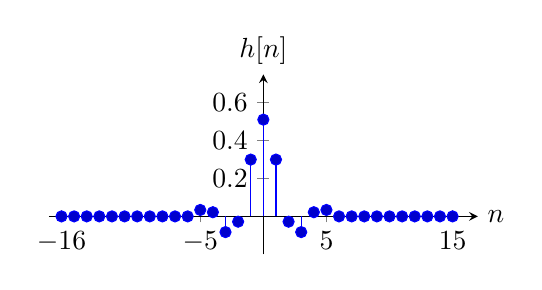
\begin{tikzpicture}
\begin{axis} [width=200pt,height=110pt,
	axis x line=middle, 
	axis y line=middle, 
	tick align=center,
	every axis x label/.style={at={(current axis.right of origin)},anchor=west},
	every axis y label/.style={at={(current axis.above origin)}, anchor=north east,above=0mm},
	xmin=-17, xmax=17,
	xtick={-16,-5, 5, 15},
	xlabel=$n$,
	ymin=-0.2, ymax=0.75,
	ytick={0, 0.2,0.4, 0.6},
	ylabel={$h [n]$},
	color=black]
\addplot+[ycomb] plot coordinates {(-16, 0.000) (-15, -0.000) (-14, -0.000) (-13, 0.000) (-12, 0.000) (-11, -0.000) (-10, -0.000) (-9, 0.000) (-8, 0.000) (-7, -0.000) (-6, -0.000) (-5, 0.034) (-4, 0.022) (-3, -0.083) (-2, -0.028) (-1, 0.300) (0, 0.511) (1, 0.300) (2, -0.028) (3, -0.083) (4, 0.022) (5, 0.034) (6, -0.000) (7, -0.000) (8, 0.000) (9, 0.000) (10, -0.000) (11, -0.000) (12, 0.000) (13, 0.000) (14, -0.000) (15, -0.000)};
\end{axis} 
\end{tikzpicture}
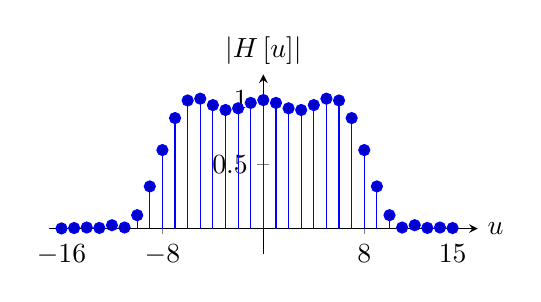
\begin{tikzpicture}
\begin{axis} [width=200pt,height=110pt,
	axis x line=middle, 
	axis y line=middle, 
	tick align=center,
	every axis x label/.style={at={(current axis.right of origin)},anchor=west},
	every axis y label/.style={at={(current axis.above origin)}, anchor=north east,above=0mm},
	xmin=-17, xmax=17,
	xtick={-16,-8,0,8,15},
	xlabel=$u$,
	ymin=-0.2, ymax=1.2,
	ylabel={$\left| H \left[ u \right] \right|$},
	color=black]
 \addplot+[ycomb]  plot coordinates {(-16, 0.001) (-15, 0.004) (-14, 0.008) (-13, 0.005) (-12, 0.026) (-11, 0.008) (-10, 0.104) (-9, 0.328) (-8, 0.611) (-7, 0.860) (-6, 0.997) (-5, 1.011) (-4, 0.961) (-3, 0.923) (-2, 0.936) (-1, 0.978) (0, 1.000) (1, 0.978) (2, 0.936) (3, 0.923) (4, 0.961) (5, 1.011) (6, 0.997) (7, 0.860) (8, 0.611) (9, 0.328) (10, 0.104) (11, 0.008) (12, 0.026) (13, 0.005) (14, 0.008) (15, 0.004)};
\end{axis}
\end{tikzpicture}
}
\caption{Hamming window ($L=5$) and the magniture of its DFT.}
%\label{fig:discretesinc}
\end{figure}
\vspace{-.2in}

In practice, when we need very small anti-aliasing filters, binomial filters are a good choice.  
The binomial filter $b_2$ has a DFT (length $N$) with a $1+\cos(2\pi/N)$ profile. At the frequency $N/4$ the gain is $1/2$. Therefore, the spectral content responsible for aliasing will not be completely removed, but the attenuation is enough in most cases.  

\vspace{-.2in}
\begin{figure}[h!]
\centerline{
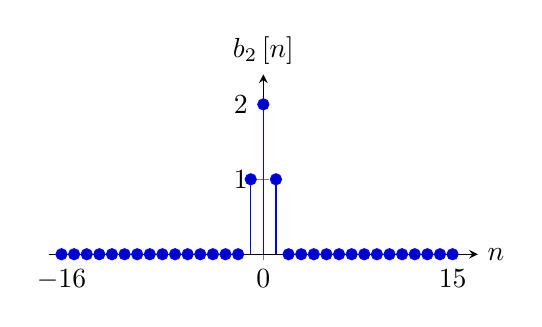
\begin{tikzpicture}
\begin{axis} [width=200pt,height=110pt,
	axis x line=bottom, 
	axis y line=middle, 
	tick align=center,
	every axis x label/.style={at={(current axis.right of origin)},anchor=west},
	every axis y label/.style={at={(current axis.above origin)}, anchor=north east,above=0mm},
	xmin=-17, xmax=17,
	xtick={-16, 0, 15},
	xlabel=$n$,
	ymin=0, ymax=2.4,
	ytick={0,...,2},
	ylabel={$b_2 \left[n\right]$}]
\addplot+[ycomb] plot coordinates {(-16,0) (-15,0) (-14,0) (-13,0) (-12,0) (-11,0) (-10,0) (-9,0) (-8,0) (-7,0) (-6,0) (-5,0) (-4,0) (-3,0) (-2,0) (-1,1) (0,2) (1,1) (2,0) (3,0) (4,0) (5,0) (6,0) (7,0) (8,0) (9,0) (10,0) (11,0) (12,0) (13,0) (14,0) (15,0)};
\end{axis} 
\end{tikzpicture}
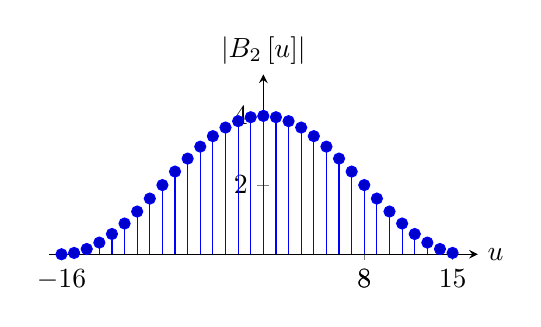
\begin{tikzpicture}
\begin{axis} [width=200pt,height=110pt,
	axis x line=middle, 
	axis y line=middle, 
	tick align=center,
	every axis x label/.style={at={(current axis.right of origin)},anchor=west},
	every axis y label/.style={at={(current axis.above origin)}, anchor=north east,above=0mm},
	xmin=-17, xmax=17,
	xtick={-16, 8, 0, 8, 15},
	xlabel=$u$,
	ymin=0, ymax=5.2,
	ytick={0,2,4},
	ylabel={$\left| B_2 \left[ u \right] \right|$},
	color=black]
 \addplot+[ycomb][domain=-16:15,samples=32,samples y=0] 
 ({x}, {abs(2+2*cos(deg(2*pi*x*1/32)))}); 
\end{axis}
\end{tikzpicture}
}
\caption{The binomial kernel $b_2 = \left[1,2,1\right]$, and its DFT.}
%\label{fig:discretesinc}
\end{figure}
\vspace{-.2in}

Or $b_4 = [ 1, 4, 6, 4, 1]$, which attenuates the aliased frequencies even more, also results in an oversmoothed signal.


%\vspace{-.2in}
\begin{figure}[h!]
\centerline{
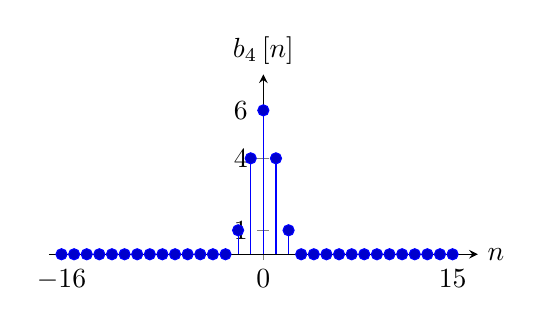
\begin{tikzpicture}
\begin{axis} [width=200pt,height=110pt,
	axis x line=bottom, 
	axis y line=middle, 
	tick align=center,
	every axis x label/.style={at={(current axis.right of origin)},anchor=west},
	every axis y label/.style={at={(current axis.above origin)}, anchor=north east,above=0mm},
	xmin=-17, xmax=17,
	xtick={-16, 0, 15},
	xlabel=$n$,
	ymin=0, ymax=7.5,
	ytick={0,1,4,6},
	ylabel={$b_4 \left[n\right]$}]
\addplot+[ycomb] plot coordinates {(-16,0) (-15,0) (-14,0) (-13,0) (-12,0) (-11,0) (-10,0) (-9,0) (-8,0) (-7,0) (-6,0) (-5,0) (-4,0) (-3,0) (-2,1) (-1,4) (0,6) (1,4) (2,1) (3,0) (4,0) (5,0) (6,0) (7,0) (8,0) (9,0) (10,0) (11,0) (12,0) (13,0) (14,0) (15,0)};
\end{axis} 
\end{tikzpicture}
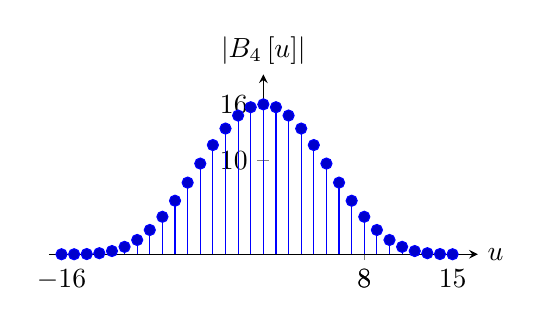
\begin{tikzpicture}
\begin{axis} [width=200pt,height=110pt,
	axis x line=middle, 
	axis y line=middle, 
	tick align=center,
	every axis x label/.style={at={(current axis.right of origin)},anchor=west},
	every axis y label/.style={at={(current axis.above origin)}, anchor=north east,above=0mm},
	xmin=-17, xmax=17,
	xtick={-16, 8, 0, 8, 15},
	xlabel=$u$,
	ymin=0, ymax=19.2,
	ytick={0, 10, 16},
	ylabel={$\left| B_4 \left[ u \right] \right|$},
	color=black]
 \addplot+[ycomb][domain=-16:15,samples=32,samples y=0] 
 ({x}, {abs(2+2*cos(deg(2*pi*x*1/32)))^2}); 
\end{axis}
\end{tikzpicture}
}
\caption{The binomial kernel $b_4 = [ 1, 4, 6, 4, 1]$, and its DFT.}
%\label{fig:discretesinc}
\end{figure}
%\vspace{-.2in}


When implementing 2D anti-aliasing filters, we apply two consecutive 1D convolutions along each dimension. 
For efficiency, the anti-aliasing filter only needs to be computed on the samples that will be kept after downsampling ($k$-strided convolution). The necessary amount of attenuation of the aliasing frequencies will have to be decided based on each application. 

\marginnote{In 2D, we can apply the binomial filter $b_2$ on each dimension, $\left[1,2,1\right]/4 \circ \left[1,2,1\right]^\transpose/4$.}[-.5in]

The images in \fig{\ref{fig:ringing_artifacts}} show the output of three different low-pass anti-aliasing filters. Note how the ideal low-pass filter introduces {\bf ringing artifacts} in the output image (\fig{\ref{fig:ringing_artifacts}}[a]). Despite that it removes frequencies that will produce aliasing after downsampling, it does that at a high cost because it introduces undesired image structures, which is exactly what we want to prevent with the anti-aliasing filter. The Hamming windowed sinc (shown in \fig{\ref{fig:ringing_artifacts}}[b]) reduces the oscillation but there is still a halo present around edges. This is because there is still one oscillation on the filter impulse response. \Fig{\ref{fig:ringing_artifacts}}{c} shows the result applying am anti-aliasing binomial filter.

%\vspace{-.2in}
\begin{figure}[h!]
\centerline{
\includegraphics[width=1\linewidth]{figures/upsamplig_downsampling/ringing_artifacts.eps}
}
\caption{Output of three different low-pass anti-aliasing filters. (left) Ideal low-pass filter. (center) Hamming window. (right) Binomial filter.}
\label{fig:ringing_artifacts}
\end{figure}
%\vspace{-.2in}

For most applications using a binomial filter ($b_2$ or $b_4$) is enough because it reduces aliasing and it does not introduce undesired image structures. 

\subsection{Downsampling}

%In order to reduce the resolution of an image, it is necessary to first apply an antialiasing filter and then to decimate the signal. 
We will call {\bf downsampling} the sequence of applying an anti-aliasing filtering followed by decimation:
\begin{align}
    z[n,m] &= \imgin \left[n,m\right] \circ h_k \left[ n,m \right]  & \quad\quad \triangleleft \quad \texttt{conv}\\
    \imgout [n,m] &= z[kn,km]  & \quad\quad \triangleleft \quad \texttt{decimation}
\end{align}

\Fig{\ref{fig:downsampling_bilinear}} shows the results when using a binomial filter as the anti-aliasing filter followed by decimation by 2, and \fig{\ref{fig:subsampled_antialiasing_textures}} shows results for different downsampling factors. 



%\vspace{-.2in}
\begin{figure}[t]
\centerline{
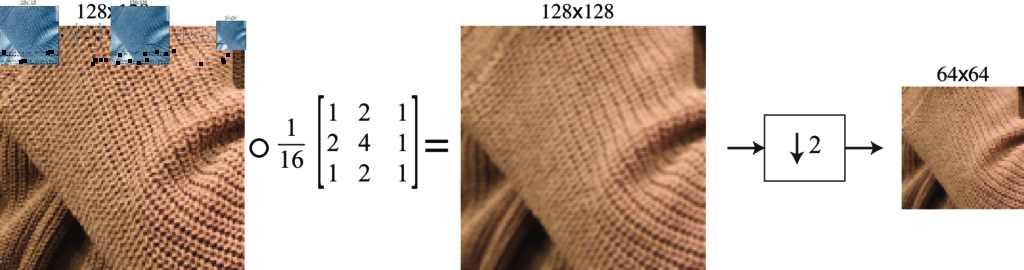
\includegraphics[width=1\linewidth]{figures/upsamplig_downsampling/downsampling_bilinear.eps}
}
\caption{Downsampling by 2 uses a binomial filter as the anti-aliasing filter followed by decimation by 2.}
\label{fig:downsampling_bilinear}
\end{figure}
%\vspace{-.2in}

In the anti-aliased downsampled images shown in \fig{\ref{fig:subsampled_antialiasing_textures}}, fine details are gone while preserving the smooth details of the image. In fact, as shown in the images below, even at $32 \times 32$, we can still see some of the orientations of the knitting pattern and the shading due to the three-dimensional shape.

%\vspace{-.2in}
\begin{figure}[t]
\centerline{
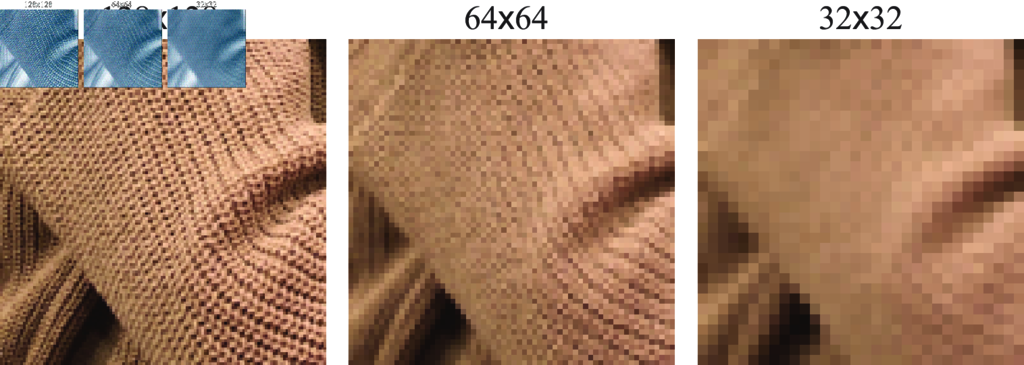
\includegraphics[width=1\linewidth]{figures/upsamplig_downsampling/subsampled_antialiasing_textures.eps}
}
\caption{Successive downsampling by a factor of 2 with anti-aliasing. Compare these results with the ones from \fig{\ref{fig:subsampled_textures}}}
\label{fig:subsampled_antialiasing_textures}
\end{figure}
%\vspace{-.2in}


As the convolution and downsampling are linear operators, sometimes it will be useful to write it as a matrix. For instance, for a 1D signal of length $N=8$  samples, if we downsample it by a factor $k=2$, then, using repeat padding for handling the boundary, and the binomial kernel as an anti-aliasing filter, we can write the downsampling operator as a matrix:
\begin{equation}
\mathbf{D}_2 = \frac{1}{4} \left[ 
\begin{array}{cccccccc}
3 & 1 & 0 & 0 & 0 & 0 & 0 & 0 \\
0 & 1 & 2 & 1 & 0 & 0 & 0 & 0 \\
0 & 0 & 0 & 1 & 2 & 1 & 0 & 0 \\
0 & 0 & 0 & 0 & 0 & 1 & 2 & 1  
\end{array}
\right]
\end{equation}

Downsampling by a factor $k=2^n$ is usually done by a sequence of $n$ stages of binomial filtering followed by downsampling by 2. Non-integer downsampling factors require an interpolation step instead of decimation.

\section{Upsampling}
\label{sec:upsampling}

%Upsampling: here we want to increase the resolution of an image. Correctly performing this operation would require making up some of the missing information. When upsampling an image, we want to do it in a way that does not introduce structures that are not present in the image.  This is an active area of research with lots of applications. In this chapter we will describe a linear operator of upsampling.

Upsampling requires increasing the resolution of an image from a low resolution image. This is a very challenging task that requires recovering information that is not available on the low resolution image. The problem of making up new details will be called super-resolution.  In this section we will focus on the simpler problem of creating an image that has $k$ times more pixels along each dimension but that contains the same amount of information than the original lower-resolution image. That is, we will not require to the upsampling procedure to predict any of the missing high-resolution details.  

Upsampling requires interpolating sample values. We want to obtain a new image $\imgout$ with more samples than the input image $\imgin$. In order to interpolate a new sample $\imgout(a,b)$, where $a$ and $b$ are continuous values, we can use different interpolations functions as we will discuss next.

\subsection{Nearest Neighbor Interpolation}
\label{sec:interpolation}


In {\bf nearest neighbor interpolation} we assign to $\imgout(a,b)$ the closest value of the input $\imgin$:
\begin{equation}
\imgout(a,b) = \imgin [ n, m ] 
\end{equation}
where $n-0.5<a<n+0.5$ and $m-0.5<b<m+0.5$. Note that here we are treating $\imgout(a,b)$ as a continuous image. Nearest neighbor interpolation results in an image that is piecewise-constant. \Fig{\ref{fig:upsampling_and_downsampling:nn_interp}} shows the nearest neighbor interpolation process graphically.
%\vspace{-.2in}
\begin{figure}[h!]
\centerline{
\includegraphics[width=1\linewidth]{figures/upsamplig_downsampling/nearest_interp2.eps}
}
\caption{Nearest neighbor interpolation in 1D and 2D.}
\label{fig:upsampling_and_downsampling:nn_interp}
%\label{fig:discretesinc}
\end{figure}
%\vspace{-.2in}

\subsection{Linear and Bilinear Interpolation}
\label{sec:bilinearinterpolation}

%{\bf Linear and bilinear interpolation}. 
{\bf Linear interpolation}: For 1D signals, the value of $\imgout(a)$ is a result of linear interpolation between the two closest input values $\imgin [n]$ and $\imgin [n+1]$, where $n<a<n+1$. 
For 2D signals, we have to interpolate the output value $\imgout(a,b)$ using four input samples: $\imgin [ n,m ]$, $\imgin [ n+1,m ]$, $\imgin [ n,m+1 ]$ and $\imgin [ n+1,m+1 ]$, where $n<a<n+1$ and $m<b<m+1$. 

{\bf Bilinear interpolation} consists of first applying linear interpolation to obtain $\imgout(a,m)$ and $\imgout(a,m+1)$ and then again applying linear interpolation between those two values to obtain $\imgout(a,b)$. The result is illustrated in \fig{\ref{fig:bilinear_interp}}.

%\vspace{-.2in}
\begin{figure}[h!]
\centerline{
\includegraphics[width=1\linewidth]{figures/upsamplig_downsampling/bilinear_interp2.eps}
}
\caption{1D linear interpolation and 2D bilinear interpolation.}
\label{fig:bilinear_interp}
\end{figure}

The linear (and bilinear) interpolations are linear operations. In the case when the upsampling factor $k$ is an integer value, the resampling operator can be efficiently implemented as a sequence of two operations: expansion and interpolation. The interpolation operation, as it is linear and spatially stationary, can be efficiently implemented as a convolution.

\marginnote{Interpolation is also a key operation when performing image warping.}

\subsection{Expansion}

Expansion by a factor $k$ consists in increasing the number of samples in the image by inserting $k-1$ zeros between each sample on the horizontal dimension, and then on the vertical dimension. This will give us the image of size $Nk \times Mk$. We will use the notation:
\begin{equation}
\img_{\uparrow k} \left[n,m\right]  = \img\left[n,m\right] \uparrow k 
\end{equation}

Expansion is a linear operator that is the transposed to the decimation operation and is defined as:
\begin{equation}
\img_{\uparrow k} \left[n,m\right] = 
 \begin{cases}
    \img \left[n/k,m/k\right]     & \quad \text{if~} \text{mod} (n,k)=0 \text{~and~} \text{mod} (m,k)=0\\
    0       & \quad \text{otherwise }\\
  \end{cases}
\label{eq:upzeros}
\end{equation}

In the 1D case, for a signal of length 4, expanding by a factor of $k=2$ can be described by the following linear operator:
\begin{equation}
\mathbf{E}_2 = \left[ 
\begin{array}{cccc}
1 & 0 & 0 & 0 \\
0 & 0 & 0 & 0\\
0 & 1 & 0 & 0\\ 
0 & 0 & 0 & 0\\
0 & 0 & 1 & 0\\ 
0 & 0 & 0 & 0\\
0 & 0 & 0 & 1\\
0 & 0 & 0 & 0
\end{array}
\right]
\end{equation}

%\subsection{Expansion in the Fourier domain}


\subsection{Interpolation Filters}

When the upsampling factor $k$ is an integer value, interpolation using the methods described in section \ref{sec:interpolation} can be implemented using a convolution. 
%The following list details the most commonly used interpolation filters. 
The interpolation filters we will discuss here are separable, so the convolution kernel can be written as the product $h\left[n,m\right] = h\left[n\right] h\left[m\right]$:

As we discussed before, there are different interpolation methods: nearest neighbor, bilinear, and so on. In this section we will study them by looking at the convolution kernel needed to implement each interpolation method. 

{\bf Nearest neighbor interpolation} consists of assigning to each interpolated sample the value of the closest sample from the input signal. This can be done by convolving the expanded image from \eqn{\ref{eq:upzeros}} with the kernel (if $k$ is even):
\begin{equation}
h  \left[n\right] =  \begin{cases}
    1     & \quad \text{if }  n \in  \left[-k/2+1, k/2\right] \\
    0       & \quad \text{otherwise }\\
\end{cases}
\end{equation}
This is very fast as it only requires replicating samples. But it gives very low quality. For $k=2$, the convolution kernel in 1D is $h  \left[n\right]=[1, 1]$

{\bf Bilinear interpolation}: As we discussed before, bilinear interpolation is done in two stages: first, linearly interpolate each sample with the two nearest neighbors across rows, and then do the same for the columns. This can also be written as a convolution with the kernel (if $k$ is even):
\begin{equation}
h  \left[n\right] =  \begin{cases}
    (k-n)/k     & \quad \text{if }  n \in \left[-k, k\right] \\
    0       & \quad \text{otherwise }\\
\end{cases}
\end{equation}
In the special case where $k=2$, the 1D bilinear interpolation kernel reduces to the binomial filter $h[n] = \left[1/2,1,1/2\right]$. And in 2D, for $k=2$, the kernel is $\left[1/2,1,1/2\right] \circ \left[1/2,1,1/2\right]^\transpose$. The binomial filter is not the best interpolation filter, but it is very efficient. When quality is important, there are better interpolation filters.  

The  plots in \fig{\ref{fig:bilinear_interp_k4}} show the nearest neighbor and linear interpolation kernels for $k=4$. 

%\marginnote{
%\vspace{-.2in}
\begin{figure}[h!]
\centerline{
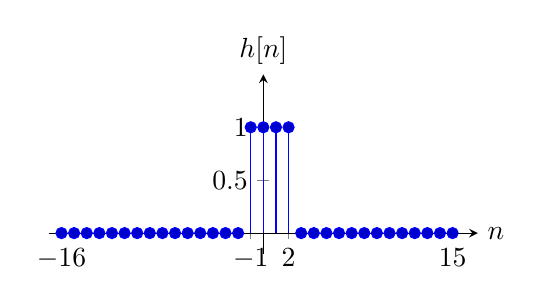
\begin{tikzpicture}
\begin{axis} [width=200pt,height=110pt,
	axis x line=middle, 
	axis y line=middle, 
	tick align=center,
	every axis x label/.style={at={(current axis.right of origin)},anchor=west},
	every axis y label/.style={at={(current axis.above origin)}, anchor=north east,above=0mm},
	xmin=-17, xmax=17,
	xtick={-16,-1, 2, 15},
	xlabel=$n$,
	ymin=-0.2, ymax=1.5,
	ytick={0, 0.5,1},
	ylabel={$h [n]$},
	color=black]
\addplot+[ycomb] plot coordinates {(-16, 0.000) (-15, -0.000) (-14, -0.000) (-13, 0.000) (-12, 0.000) (-11, -0.000) (-10, -0.000) (-9, 0.000) (-8, 0.000) (-7, -0.000) (-6, -0.000) (-5, 0) (-4, 0) (-3, 0) (-2, 0) (-1, 1) (0, 1) (1, 1) (2, 1) (3, 0) (4, 0) (5, 0.0) (6, 0.000) (7, -0.000) (8, 0.000) (9, 0.000) (10, 0.000) (11, 0.000) (12, 0.000) (13, 0.000) (14, 0) (15, 0.000)};
\end{axis} 
\end{tikzpicture}
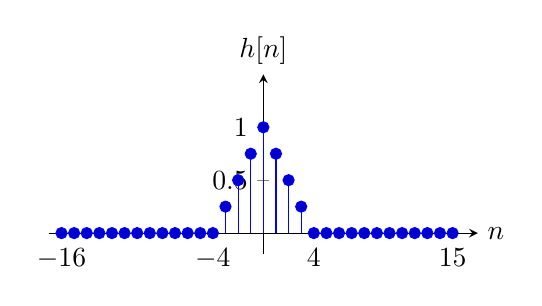
\begin{tikzpicture}
\begin{axis} [width=200pt,height=110pt,
	axis x line=middle, 
	axis y line=middle, 
	tick align=center,
	every axis x label/.style={at={(current axis.right of origin)},anchor=west},
	every axis y label/.style={at={(current axis.above origin)}, anchor=north east,above=0mm},
	xmin=-17, xmax=17,
	xtick={-16,-4, 4, 15},
	xlabel=$n$,
	ymin=-0.2, ymax=1.5,
	ytick={0, 0.5,1},
	ylabel={$h [n]$},
	color=black]
\addplot+[ycomb] plot coordinates {(-16, 0.000) (-15, -0.000) (-14, -0.000) (-13, 0.000) (-12, 0.000) (-11, -0.000) (-10, -0.000) (-9, 0.000) (-8, 0.000) (-7, -0.000) (-6, -0.000) (-5, 0) (-4, 0) (-3, 1-3/4) (-2, 1-2/4) (-1, 1-1/4) (0, 1) (1, 1-1/4) (2, 1-2/4) (3, 1-3/4) (4, 0) (5, 0.0) (6, 0.000) (7, -0.000) (8, 0.000) (9, 0.000) (10, 0.000) (11, 0.000) (12, 0.000) (13, 0.000) (14, 0) (15, 0.000)};
\end{axis} 
\end{tikzpicture}
}
\caption{Kernels for (left) nearest neighbor, and (right) linear interpolation for $k=4$.}
\label{fig:bilinear_interp_k4}
\end{figure}

Other popular interpolation methods are the {\bf bicubic interpolation} and the {\bf Lanczos interpolation}. 

%\item Ideal interpolation:



\subsection{Upsampling}

Upsampling consists in the sequence of expansion followed by interpolation:
\begin{align}
    z \left[n,m\right] &= \imgin \left[n,m\right] \uparrow k 
% \begin{cases}
%    x \left[n/k,m/k\right]     & \quad \text{if } mod(n,k)=0 \text{~and~} mod(m,k)=0\\
%    0       & \quad \text{otherwise }\\
%  \end{cases}
  & \quad\quad \triangleleft \quad \texttt{expansion}\\
    \imgout [n,m] &= z \left[n,m\right] \circ h_k \left[n,m\right]  & \quad\quad \triangleleft \quad \texttt{conv}
\end{align}



Upsampling by a factor of 2 is done by inserting one 0 between each two samples (first for the horizontal dimension and then for the vertical one), and then interpolating between samples applying the binomial filter $\left[1/2,1,1/2\right] \circ \left[1/2,1,1/2\right]^\transpose$. 

\Fig{\ref{fig:upsamplingazebra}} shows the upsampling process for a color image. Each color channel is upsampled by a factor of $k=2$ independently. The top row shows the input image, the expanded image by inserting zeros between samples, the binomial kernel and the resulting interpolated image. The bottom row shows the magnitude of DFTs of each corresponding image. Note that the binomial interpolation filter does not completely suppress  the copies of the original DFT that appear when inserting new samples. Remember that the DFTs have the same number of samples as the corresponding input image. The DFT of the kernel is shown by zero padding the convolutional kernel to match the image size. Despite that this interpolation does correspond to an ideal interpolation filter (a sinc) the interpolated image looks reasonably good.

%The convolution (eq.~\ref{eq:up_interp}) only needs to be computed on the samples to be interpolated. In this example, you could convolve the rows of the original image with the filter $\left[1,1\right]/2$ and then create a new signal taking one pixel from the original image and one pixel from the result of this convolution. Then repeat the same operation with the columns. Note that upsampling uses a low resolution version of the input signal to increase the amount of samples! This is certainly something very different to super-resolution where we want to create an image that looks sharper. 


\begin{figure}[t]
\includegraphics[width=1\linewidth]{figures/upsamplig_downsampling/upsampling_bilinear.eps}
\caption{Upsampling by a factor of $k=2$ using a bilinear interpolation filter.} 
\label{fig:upsamplingazebra}
\end{figure}



The upsampling operator is also a linear operation, therefore we can also write it in matrix form. For instance, for a 1D signal of length $N=4$  samples, if we upsample it by a factor $k=2$, then, using repeat padding for handling the boundary and the bilinear interpolation, we can write the upsampling operator as a matrix:
\begin{equation}
\mathbf{U}_2 = \left[ 
\begin{array}{cccc}
1    & 0    & 0  & 0\\
0.5  & 0.5  & 0  & 0\\
0    & 1    & 0  & 0\\
0    & 0.5 & 0.5 & 0\\
0    & 0    & 1  & 0\\
0    & 0    & 0.5& 0.5\\
0    & 0    & 0  & 1\\
0    & 0    & 0  & 1
\end{array}
\right]
\end{equation}

Multiplying this matrix by a signal of length 4, gives an output signal of length 8. The output samples at locations 1, 3, 5, 7, and 8 are copies of the input samples 1, 2, 3, and 4, while samples 2, 4, and 6 are computed as the average of two consecutive input samples. The last output sample is a copy of the last input sample because it corresponds to extending the input using repeat padding.



%\section{Translation invariance and the importance of anti-aliasing filtering}


\section{Concluding Remarks}

Aliasing is a constant source of problems in many image processing pipelines. In computer vision, aliasing can introduce noise, spurious features and textures, and lack of translation invariance. In \chap{\ref{chapter:convolutional_neural_nets}} we will discuss how aliasing affects the quality of some of the convolutional layers used in neural networks. 

Some of the tools we discussed in this chapter will also be used in other settings such as when building image pyramids (\chap{\ref{chapter:image_pyramids}}), and geometry (\chap{\ref{chapter:geometry_homogeneous}}).

Aliasing is often a source of image artifacts in generative image models. One example are generative adversarial networks (\chap{\ref{chapter:generative_models}}) where images are produced as a sequence of learned convolutions and upsampling stages. When the upsampling operations are done without paying attention to aliasing, the output images show a number of artifacts as has been shown in \cite{Karras2021}. Those artifacts can be removed by carefully implementing each stage to avoid aliasing. 

